\documentclass[letterpaper,12pt]{article}

% @@@@@@@@@@@@@@@@@@@@@@@@@@@@@@@@@@@@@@@@@@@@@@@@@@@@@@@@@@@@>
% VALORES A MODIFICAR POR USTED:
% @@@@@@@@@@@@@@@@@@@@@@@@@@@@@@@@@@@@@@@@@@@@@@@@@@@@@@@@@@@@>

% NOTE: Leer nota en el README sobre la font.

\newcommand{\titulo}{Título de la memoria}
\newcommand{\ciudad}{Valparaíso} % e.g. Valparaíso
% TODO: Consultar el formato de los nombres:
\newcommand{\nombrealumno}{Ricardo Gamboa Arias}
\newcommand{\nombreprofesor}{Elizabeth Montero}
\newcommand{\nombrecorreferente}{Nombre del correferente}
% Mes y año del examen
\newcommand{\mesexamen}{Diciembre}
\newcommand{\anioexamen}{2018}
% Dedicatoria y agradecimientos
\newcommand{\dedicatoria}{

}
\newcommand{\agradecimientos}{

}
\newcommand{\resumen}{

}
\newcommand{\resumeningles}{

}
\newcommand{\palabrasclave}{

}
\newcommand{\palabrasclaveingles}{

}
% @@@@@@@@@@@@@@@@@@@@@@@@@@@@@@@@@@@@@@@@@@@@@@@@@@@@@@@@@@@@>

% Paquete para importar imágenes
\usepackage{graphicx}
% Directorio de las imágenes
\graphicspath{ {figures/} }

% Idioma y fuentes
\usepackage[spanish,es-tabla]{babel}
\usepackage[T1]{fontenc}
\usepackage{fontspec}
% Paquete para definir cualquier tamaño de font
\usepackage{anyfontsize}

% Seleccionar font
\setmainfont{Carlito}

% Tamaño de la página y márgenes
\usepackage[letterpaper,top=2.5cm,bottom=3cm,left=3cm,right=3cm,marginparwidth=1.75cm]{geometry}

% Determinar entrelineado:
\renewcommand{\baselinestretch}{1.0}

% Eliminar sangrías:
\setlength{\parindent}{0cm}

% Paquete para definir los formatos de los títulos
\usepackage[explicit]{titlesec}

\titleformat{name=\section}[block]{\fontsize{16}{24}\selectfont\bfseries}{}{0pt}{#1}
\titleformat{name=\section,numberless}[block]{\fontsize{16}{24}\selectfont\bfseries}{}{0pt}{#1}
\titlespacing*{name=\section}{0pt}{0pt}{0.5cm}
\titlespacing*{name=\section,numberless}{0pt}{0pt}{0.5cm}

% Separación entre parrafos
\setlength{\parskip}{0.4cm}

% Paquetes de utilidad general
\usepackage{amsmath}
\usepackage{graphicx}
\usepackage{float}
\usepackage[colorlinks=true, allcolors=blue]{hyperref}
\usepackage{breakcites}
\usepackage{listings}

% Formato de las tablas de contenido
\usepackage[tocflat]{tocstyle}
\usetocstyle{allwithdot}

% Para obtener el número de la última página
\usepackage{lastpage}

% Header y footer
\usepackage{fancyhdr}
\fancypagestyle{portada}{
    \lhead{}
    \chead{}
    \rhead{}
    \lfoot{}
    \cfoot{\fontsize{10}{12}\selectfont \thepage}
    \rfoot{}
    \renewcommand{\headrulewidth}{0pt}
}
\fancypagestyle{intermedio}{
    \lhead{}
    \chead{\fontsize{10}{12}\selectfont\MakeUppercase{\titulo}}
    \rhead{}
    \lfoot{}
    \cfoot{\fontsize{10}{12}\selectfont Página \textbf{\thepage}\ de \textbf{\pageref{LastPage}}}
    \rfoot{}
    \renewcommand{\headrulewidth}{1pt}
}

% Comandos para secciones
\newcommand{\secnumbersection}[1]{
\addtocounter{section}{1}
\section*{CAPÍTULO \thesection \texorpdfstring{\\}\ #1}
\addcontentsline{toc}{section}{CAPÍTULO \thesection : #1}
\setcounter{subsection}{0}
}
\newcommand{\secnumberlesssection}[1]{
\section*{#1}
\phantomsection
\addcontentsline{toc}{section}{#1}
\setcounter{subsection}{0}
}

% Nombres
\addto\captionsspanish{\renewcommand{\contentsname}{ÍNDICE DE CONTENIDOS}}
\addto\captionsspanish{\renewcommand{\listfigurename}{ÍNDICE DE FIGURAS}}
\addto\captionsspanish{\renewcommand{\listtablename}{ÍNDICE DE TABLAS}}
\makeatletter
\renewenvironment{thebibliography}[1]
     {\secnumberlesssection{REFERENCIAS BIBLIOGRÁFICAS}
      \@mkboth{\MakeUppercase\bibname}{\MakeUppercase\bibname}%
      \list{\@biblabel{\@arabic\c@enumiv}}%
           {\settowidth\labelwidth{\@biblabel{#1}}%
            \leftmargin\labelwidth
            \advance\leftmargin\labelsep
            \@openbib@code
            \usecounter{enumiv}%
            \let\p@enumiv\@empty
            \renewcommand\theenumiv{\@arabic\c@enumiv}}%
      \sloppy
      \clubpenalty4000
      \@clubpenalty \clubpenalty
      \widowpenalty4000%
      \sfcode`\.\@m}
     {\def\@noitemerr
       {\@latex@warning{Empty `thebibliography' environment}}%
      \endlist}
\makeatother

% Personalizar Tabla de Contenidos

\usepackage{tocloft}
\renewcommand{\cftsecfont}{\fontsize{12}{14}\selectfont\fontspec{Carlito}}
\renewcommand{\cftsubsecfont}{\fontsize{12}{14}\selectfont\fontspec{Carlito}}
\renewcommand{\cftsubsubsecfont}{\fontsize{12}{14}\selectfont\fontspec{Carlito}}

\renewcommand\cftfigfont{\fontsize{12}{14}\selectfont\fontspec{Carlito}}

% Links sin color
\usepackage{hyperref}
\hypersetup{colorlinks = false}

% @@@@@@@@@@@@@@@@@@@@@@@@@@@@@@@@@@@@@@@@@@@@@@@@@@@@@@@@@@@@>
\begin{document}

\pagestyle{portada}
\pagenumbering{roman}
% NOTE: Este archivo contiene la portada, la dedicatoria, los agradecimientos y el resumen.
% __NO ES NECESARIO MODIFICAR ESTE ARCHIVO__, esas se modifican con los comandos que aparecen en main.tex
%@@@@@@@@@@@@@@@@@@@@@@@@@@@@@@@@@@@@@@@@@@@@@@@@@@@@@@@@@@@@@@
\begin{titlepage}
\begin{center}
\noindent
{\fontsize{18}{22}\selectfont UNIVERSIDAD TÉCNICA FEDERICO SANTA MARÍA \\}
{\fontsize{16}{19}\selectfont DEPARTAMENTO DE INFORMÁTICA \\}
{\fontsize{16}{19}\selectfont \MakeUppercase{\ciudad}\ - CHILE \\}
\vspace{1.5cm}

\includegraphics[width=4.41cm,height=3.34cm]{logo/logo.jpg} \\
\vspace{1.5cm}
{\fontsize{20}{24}\selectfont ``\MakeUppercase{\titulo}'' \\}
\vfill
{\fontsize{16}{19}\selectfont \MakeUppercase{\nombrealumno} \\}
\vfill
{\fontsize{16}{19}\selectfont MEMORIA PARA OPTAR AL TÍTULO DE \\}
{\fontsize{16}{19}\selectfont INGENIERO CIVIL EN INFORMÁTICA \\}
\vspace{1.5cm}
{\fontsize{14}{17}\selectfont Profesor Guía: \nombreprofesor \\}
{\fontsize{14}{17}\selectfont Profesor Correferente: \nombrecorreferente \\}
\vspace{2.5cm}
{\fontsize{14}{17}\selectfont \mesexamen\ - \anioexamen \\}
\end{center}
\end{titlepage}

%@@@@@@@@@@@@@@@@@@@@@@@@@@@@@@@@@@@@@@@@@@@@@@@@@@@@@@@@@@@@@@
\newpage
\setcounter{page}{2}
\
\vfill
\vfill
\begin{flushright}
\noindent {\fontsize{16}{19}\selectfont \textbf{DEDICATORIA} \\}
\end{flushright}
\begin{flushright}
\noindent \dedicatoria
\end{flushright}
\vfill
%@@@@@@@@@@@@@@@@@@@@@@@@@@@@@@@@@@@@@@@@@@@@@@@@@@@@@@@@@@@@@@
\newpage
\begin{center}
\noindent {\fontsize{16}{19}\selectfont \textbf{AGRADECIMIENTOS} \\}
\end{center}
\noindent \agradecimientos
\vfill
%@@@@@@@@@@@@@@@@@@@@@@@@@@@@@@@@@@@@@@@@@@@@@@@@@@@@@@@@@@@@@@
\newpage
\secnumberlesssection{RESUMEN}
\vspace{0.3cm}
\noindent \textbf{Resumen---}\resumen \ \\
\vspace{0.3cm} \\
\noindent \textbf{Palabras Clave---}\palabrasclave \ \\
% @@@@@
\vspace{1.2cm} \\
% @@@@@
%\noindent {\fontsize{16}{19}\selectfont \textbf{ABSTRACT}}
%\vspace{1.2cm} \\
\secnumberlesssection{ABSTRACT}
\vspace{0.3cm}
\noindent \textbf{\emph{Abstract}---}\resumeningles \ \\
\vspace{0.3cm} \\
\noindent \textbf{\emph{Keywords}---}\palabrasclaveingles \ \\
%@@@@@@@@@@@@@@@@@@@@@@@@@@@@@@@@@@@@@@@@@@@@@@@@@@@@@@@@@@@@@@


\newpage
\secnumberlesssection{GLOSARIO}

{\setlength{\parskip}{0cm} % Para evitar saltar entre cada elemento nombrado.
%Colocar aquí siglas:
Agente: Entidad que tiene que moverse por el tablero.

Heuristica: Método diseñado para resolver un problema mas rápido cuando los métodos clásicos tienen algún problema en el caso especifico. Normalmente sacrifica optimalidad, completitud, precision o validez para lograrlo.

Tablero: Representación computacional en forma de grafo que se en la representación del problema y la búsqueda de la solución.
}


%Índice de contenidos:
\newpage
\thispagestyle{portada}
\tableofcontents

%Índice de figuras:
\newpage
\thispagestyle{portada}
\phantomsection
\addcontentsline{toc}{section}{ÍNDICE DE FIGURAS}
\listoffigures
\phantomsection
\addcontentsline{toc}{section}{ÍNDICE DE TABLAS}
\listoftables

\newpage
\pagestyle{intermedio}
\pagenumbering{arabic}
\secnumberlesssection{INTRODUCCIÓN}



\newpage
\secnumbersection{DEFINICIÓN DEL PROBLEMA}

\subsection{CONTEXTO}

Durante años hemos necesitado encontrar el camino para llegar desde un lugar a otro, la velocidad con la que se obtiene esta información puede ser de gran ayuda en casos como encontrar el camino a un lugar con un GPS o encontrar un camino optimizado para un robot.
Problema del camino más corto es un problema de la teoría de grafos que quiere encontrar un camino con una característica menor, en nuestro caso es tiempo de viaje.
En casos donde el algoritmo no es lo suficientemente rápido se pueden usan atajos para obtener soluciones menos óptimas pero que son mas rápidas de obtener.

\subsection{PROBLEMA}

\textit{Pathfinding}, es una rama del problema del camino mas corto, se basa en buscar el camino entre dos puntos en un espacio representado computacionalmente(Ver figura \ref{fig:example}). Se busca una lista de posiciones por las cuales tenga que pasar el agente\footnote{Entidad que tiene que moverse por el tablero.} de tal modo que se simplifique el movimiento a saltos entre posiciones como en un tablero o movimientos simples como lineas rectas que pueda seguir el agente.

\begin{figure}[h]
\centering
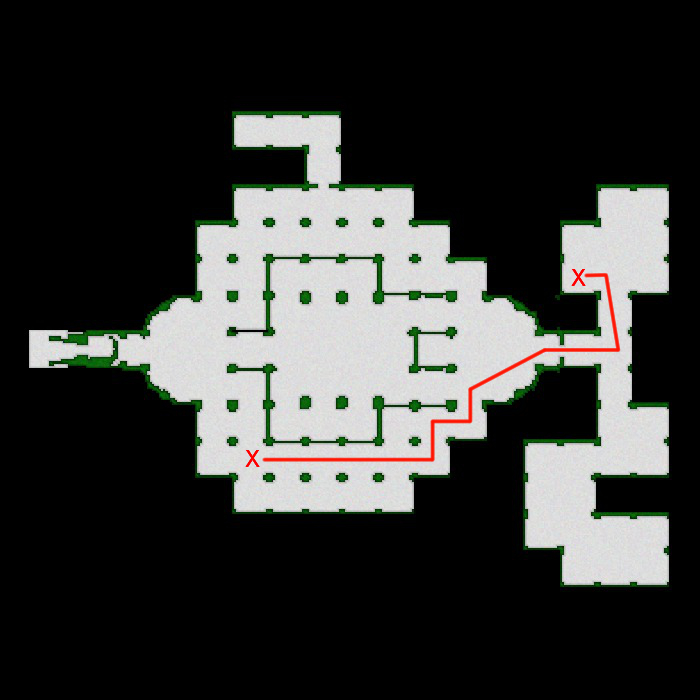
\includegraphics[width=0.8\textwidth]{example}
\caption{\label{fig:example} Ejemplo de \textit{pathfinding}} Fuente: \textit{Dragon Age: Origins}\cite{bioware2009pathfinding}.
\end{figure}

\subsection{DIFERENCIAS}

\subsubsection{TABLERO}

Dependiendo del tipo de tablero en el que tiene encontrar un camino se encuentran distintos problemas, estos se separan en:

\begin{itemize}
    \item Estático: El único movimiento en el tablero es el agente que esta buscando el camino, este es el caso mas simple porque no se tiene que ajustar el \textit{pathfinding} durante el movimiento.
    \item Dinámico: Existen cambios en el tablero provocados por otras entidades o otros efectos. En este caso el problema es que el camino encontrado con anterioridad puede parar de ser funcional de un momento a otro y buscar el camino completamente después de cada movimiento es demasiado costoso.
\end{itemize}

También existen problemas donde se puede encontrar el camino para distintos tipos de agentes que se relacionan diferente con los distintos tipos de terreno, por ejemplo, agentes que puedan desplazarse sobre el agua no tienen que preocuparse de esquivarla.

\subsubsection{VISIBILIDAD}

Otro punto a considerar es el conocimiento previo del tablero y la visibilidad que se tiene de este, si el tablero es conocido, se pueden usar algoritmos que permiten optimizar el \textit{pathfinding} con procesamiento previo, estos se separan en:

\begin{itemize}
    \item Conocimiento total del tablero: El agente conoce el tablero y tiene visión de este en cada momento.
    
    \item Conocimiento del tablero pero visibilidad reducida: El agente tiene alguna especie de cámara o visión periférica por lo cual conoce los cambios en el tablero que están cerca de el.
    
    \item Conocimiento reducido: No hay conocimiento del tablero y este se genera con la visión del agente mientras se esta moviendo.
\end{itemize}

\subsubsection{MOVIMIENTO}

El movimiento del agente puede ser variable dependiendo del terreno por lo cual puede variar el tiempo o el coste\footnote{En juegos con turnos, los agentes tienen una cantidad de puntos para sus movimientos que se reducen dependiendo del terreno por el que caminan}. También el movimiento puede separarse en:

\begin{itemize}
    \item Discreto: En juegos con tablero se usa este tipo de movimiento porque las posiciones posibles están dadas por enteros, como en el ajedrez.
    
    \item Continuo: En el trabajo de robótica y en juegos en tiempo real se usan movimientos continuos, para encontrar el camino el mundo continuo se reduce a un sistema discreto y luego con ese sistema se puede crear el movimiento continuo.
\end{itemize}

\subsubsection{TAMAÑO}

Cuando tienes que mover distintos agentes dentro de un tablero, pueden existir agentes que ocupan mas espacio que otros por lo cual sus caminos tienen que poder contenerlos. Casos como unidades que ocupan 1 celda del tablero y otras que ocupan 4 puedes ser mas complicados de tratar en un solo grafo.


\subsection{GRAFOS}

La representación que se usara en la memoria son grafos, un conjunto de nodos unidos por arcos que permiten relacionar a estos. Estos nodos son las posibles posiciones en el espacio y los arcos representan las formas de movimiento entre ellos.
Los arcos llevan un valor agregado que nos permite saber cuanto cuesta el movimiento desde un punto a otro, en un tablero de cuadrados existen 4 u 8 formas de movimiento dependiendo de como sea la decisión de diseño(Ver figura \ref{fig:example2}). Los movimientos cardinales tienen un coste 1 y los diagonales tienen un coste $ \sqrt{2} $.
Se explicara mas a fondo en el Marco Conceptual.


\begin{figure}[h]
\centering
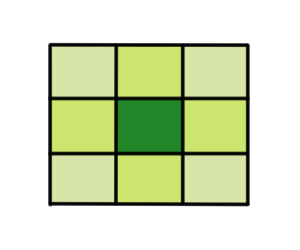
\includegraphics[width=0.5\textwidth]{example2}
\caption{\label{fig:example2} Ejemplo de movimiento entre Nodo central, sus cuatro direcciones cardinales y las diagonales en colores diferentes.} Fuente: Propio.
\end{figure}

\subsection{ENFOQUE}

En esta memoria nos centraremos en el problema de \textit{pathfinding} en juegos en tiempo real, por lo cual los dos problemas principales que se enfrentan son:

\begin{itemize}

    \item Tiempo: En los juegos normalmente se le permite un tiempo a la búsqueda de caminos de algunos mili segundos para no entorpecer el funcionamiento del resto de las funciones del juego por lo cual la velocidad de el algoritmo se vuelve imperativa para que la calidad del juego no sea afectada.
    
    \item Calidad: Dentro del tiempo que es posible ocupar se tiene que entregar la mejor solución posible de tal modo que los agentes no tomen caminos que podrían ser denominados de poco humano para los jugadores.
    
\end{itemize}

Además nos estamos enfocado en mapas auto generados\footnote{Creados en el momento que se inicia la partida} no podemos usar pre-procesamiento para obtener un aumento de velocidad en el \textit{pathfinding}, por lo cual nos enfrentamos a un problema que no permite ocupar pre-procesamiento directamente. 

\subsection{OBJETIVO DE LA SOLUCIÓN}


\subsubsection{OBJETIVOS GENERALES}


\subsubsection{OBJETIVOS ESPECÍFICOS}


\begin{enumerate}
    \item  
    \item
    \item
\end{enumerate}
\newpage
\secnumbersection{MARCO CONCEPTUAL}

\subsection{PATHFINDING}

\textit{Pathfinding} es la creación de un plan de acción para cursar la ruta mas corta entre dos puntos, usando computación. El exponente inicial para la solución de este problema es el algoritmo de \textit{Dijkstra's} que encuentra la ruta optima en un grafo con costos en sus arcos desde un nodo a todos los otros.

En el trabajo con videojuegos se acostumbra a usar estos \textit{benchmarks} estandarizados \cite{sturtevant2012benchmarks}, estos han sido extraídos de juegos o creados para poner a prueba las distintas formas de encontrar la solución.

Es un punto importante del trabajo en videojuegos por la demanda de eficiencia, el trabajo desarrollado para el \textit{pathfinding} regularmente tiene un tiempo alocado que no permite buscar indefinidamente los caminos por lo cual es necesario tener medidas que han ido cambiando con los años para obtener resultados en el tiempo esperado, muchas veces esto genera agentes que se mueven de maneras innaturales pero entregarle mas tiempo a esto no es posible porque afectaría el desempeño del juego.

Normalmente se tienen que mover varios agentes en tiempo real y para esto existen distintos algoritmos. Antes de entrar a hablar de los distintos algoritmos, veremos un poco de la historia y teoría ocupada.

\subsection{TEORIA DE GRAFOS}

\subsubsection{DEFINICION DE GRAFO}

Un grafo G consiste en un grupo no vació, finito de nodos, $V(G)$, y un grupo finito de arcos de pares de nodos, $E(G)$. Un vértice \{v,w\}, uno los vértices $v$ y $w$. Se abrevia $vw$.

Los grafos que consideraremos serán mas simples porque no consideran mas de un arco entre los mismos dos nodos y no tienen arcos de un nodo a si mismo

La Figura \ref{fig:graph} muestra el grafo $G$, donde $V(G) = \{u,v,w,z\}$ y $E(G) = \{uv,uw,vw,wz\}$

\begin{figure}[h]
\centering
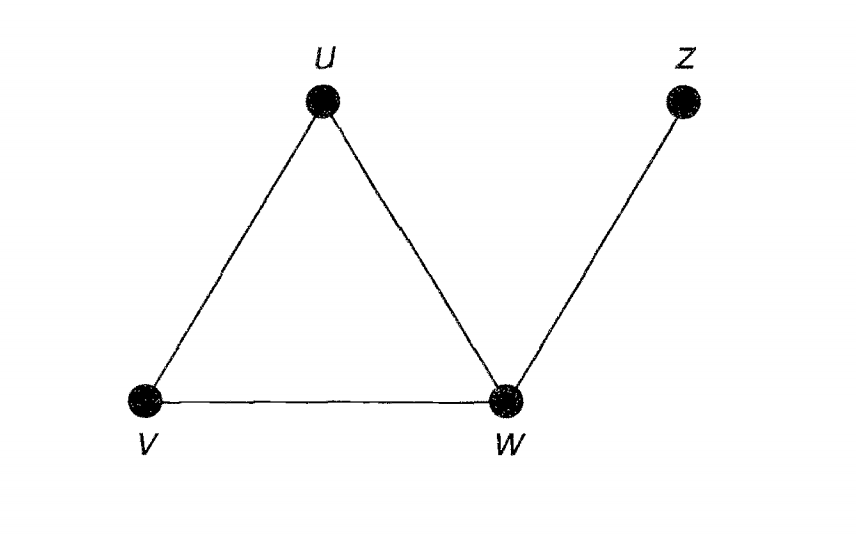
\includegraphics[width=0.5\textwidth]{grafo}
\caption{\label{fig:graph} Ejemplo de Grafo} Fuente: \textit{Introduction to Graph Theory} \cite{wilson1970introduction}.
\end{figure}

\subsubsection{CAMINO}

Un camino en un grafo $G$ es una secuencia finita de de arcos denotado por $v_o \rightarrow v_1 \rightarrow v_2 \rightarrow v_3 \rightarrow v_4 \rightarrow v_5...$

La Figura \ref{fig:graph2} muestra el grafo $G$, donde $V(G) = \{x,v,w,y,z\}$ y $E(G) = \{vx,vw,vy,wx$ $,wy,yx,xz,yz,zz\}$. Se pueden generar distintos caminos entre $v$ y $z$, de distintos largos, por ejemplo:

\begin{itemize}
\item $v \rightarrow w \rightarrow x \rightarrow z$ con largo 3.
\item $v \rightarrow y \rightarrow z$ con largo 2.
\end{itemize}

\begin{figure}[h]
\centering
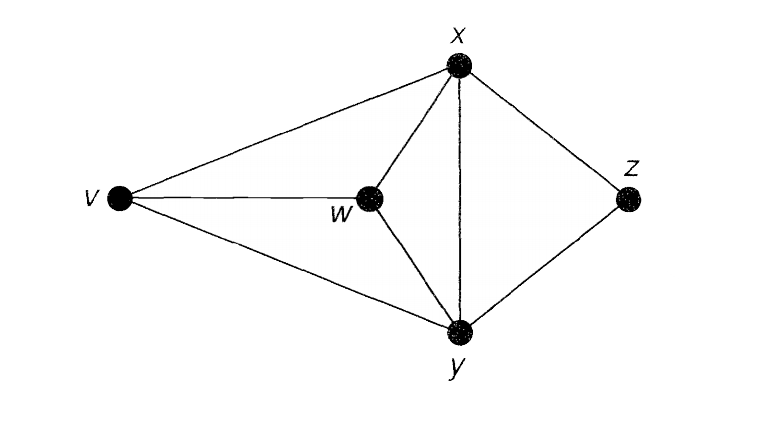
\includegraphics[width=0.5\textwidth]{grafo2}
\caption{\label{fig:graph2} Ejemplo de Camino en un Grafo} Fuente: Introduction to Graph Theory \cite{wilson1970introduction}.
\end{figure}

\subsubsection{COSTO}

Los arcos de los grafos que ocuparemos tendrán asociados un valor que llamaremos costo, donde el arco entre v y w se representa $\{v,w,X\}$ con $X \in \mathcal{R}^+ $

La Figura \ref{fig:graph3} muestra el mismo grafo anterior con valores en los arcos y compararemos los caminos mostrados antes, ahora con el costo total asociado.

\begin{itemize}
\item $v \rightarrow w \rightarrow x \rightarrow z$ con costo 3.
\item $v \rightarrow y \rightarrow z$ con costo 5.
\end{itemize}

En estos caminos podemos observar que el camino con menos arcos, no es mejor y esto es interesante cuando empezamos a trabajar en \textit{pathfinding}.

\begin{figure}[h]
\centering
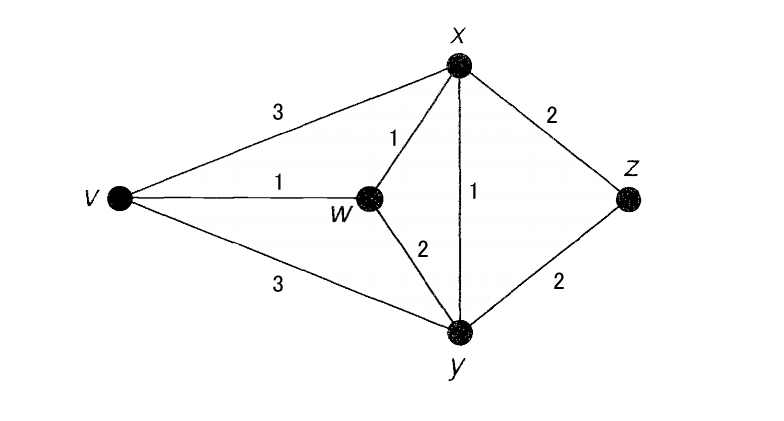
\includegraphics[width=0.5\textwidth]{grafo3}
\caption{\label{fig:graph3} Ejemplo de Camino en un Grafo con Costo en sus arcos} Fuente: \textit{Introduction to Graph Theory} \cite{wilson1970introduction}, con edición propia.
\end{figure}

\subsection{ALGORITMOS}

Los métodos de \textit{pathfinding}, comúnmente necesitan tres cosas. Un grafo para representar el mapa, un algoritmo de búsqueda y una heuristica para guiar la búsqueda.\cite{botea2013pathfinding}

Una forma muy común de representar los mapas, es en casillas como el ajedrez, que se consideran de forma atómica\footnote{El movimiento hacia dentro y fuera de la casilla se considera una acción por la búsqueda, no hay movimientos mas pequeños.}. Esta representación como grafo te permite aplicar el algoritmo de búsqueda.

Un primer acercamiento a un algoritmo para buscar un camino optimo es probar con todos los posibles caminos, esto se podría lograr con una búsqueda en profundidad. Pero se pueden eliminar caminos imposibles con anterioridad, o buscar en caminos mas problemas antes, por lo cual se usan heuristicas para acelerar la búsqueda.

Ahora entramos a hablar mas en detalle de los distintos algoritmos y heuristicas comúnmente ocupados para este problema.

\subsubsection{DIJKSTRA'S}

El algoritmo de \textit{Dijkstra's} \cite{dijkstra1959note} encuentra el camino mas corto entre dos nodos. Empieza con el nodo inicial y sus vecinos en un conjunto de opciones, en cada iteraccion selecciona el nodo con la menor distancia al inicial del conjunto de opciones, este queda marcado como visitado y sus vecinos que no han sido visitados entran al conjunto de opciones. Se repite este proceso hasta encontrar el nodo final o que este vacio el conjunto de opciones, en tal caso no existe un camino entre los nodos.

La primera version entregaba la distancia del camino, pero posteriores iteraciones han entregado el camino a todos los otros nodos desde el inicial o el camino a un nodo especifico entregado.
\newline

\begin{figure}[h]
\centering
\begin{lstlisting}[frame=single]
function Dijkstra(Graph, source):
    for each vertex v in Graph:      	// Inicializar
        dist[v] := infinity             //Dist. Desconocida
        previous[v] := undefined        // Nodo desconocido
    dist[source] := 0 	                // Nodo inicial
    Q := the set of all nodes in Graph 	// Nodos a recorrer
    while Q is not empty:               // Main loop
        u := node in Q with smallest dist[ ]
        remove u from Q
        for each neighbor v of u:       // Vecinos faltantes
            alt := dist[u] + dist_between(u, v)
            if alt < dist[v]            // Usar Dist. menor
                dist[v] := alt
                previous[v] := u
    return previous[ ]
\end{lstlisting}
\caption{\label{fig:dijisCode} Pseudo Codigo de algoritmo de \textit{Dijstra's}} Fuente: GITTA \cite{Brilliant2009April}.
\end{figure}


La Figura \ref{fig:djis} se muestra un grafo al que se le aplica este algoritmo para encontrar todos los caminos mínimos a el resto de sus nodos.


\begin{figure}[h]
\begin{minipage}[c]{0.5\textwidth}
	\centering
    Antes de la Búsqueda
	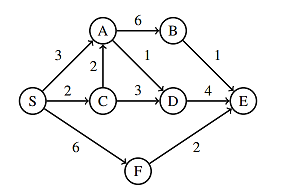
\includegraphics[width=1\textwidth]{djis1}
\end{minipage}
\begin{minipage}[c]{0.5\textwidth}
	\centering
    Después de la Búsqueda
	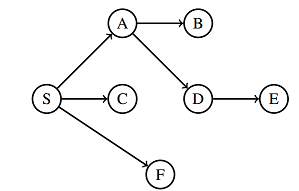
\includegraphics[width=1\textwidth]{djis2}
\end{minipage}
\caption{\label{fig:djis} Ejemplo de la aplicacion del algoritmo de Djkstra's} \begin{center}
	Fuente: \textit{Dijkstra's Shortest Path Algorithm} \cite{Brilliant2009April}.
\end{center}
\end{figure}

Cabe destacar que el algoritmo de \textit{Dijstra's} no funciona si existen arcos con costos negativos, pero esto no afecto a la búsqueda de caminos porque no tendría sentido que el agente se demorara un tiempo negativo en una acción.


\subsubsection{A*}

A* es una variación de \textit{Dijkstra's}, usa una heuristica que permite moverse a los nodos que están en dirección al objetivo. Logra esto sumando el peso del arco con una suposición de la distancia del nodo siguiente al nodo objetivo.

Esta suposición de la distancia es la heuristica, esta permite que no se revisen caminos posiblemente mas largos cuando existe la posibilidad de que exista un camino directo. 

El Seudo Codigo de A* es similar a Dijkstra's, el cambio a destacar es la diferencia que genera la heuristica(Como se ve en la figura \ref{fig:ACode}), en el ejemplo posterior estamos usando:

\begin{align*}
	heuristic(v,f) &= |v.x - f.x| + |v.y - f.y| \\
	v &= vertice\  actual \\
	f &= vertice\ final \\
	t.x &= posicion\ x\ en\ el\ tablero\ de\ vertice\ t \\
	t.y &= posicion\ y\ en\ el\ tablero\ de\ vertice\ t 
\end{align*}

	



\begin{figure}
\centering
\begin{lstlisting}[frame=single]
function A*(Graph, source, heuristic):
    for each vertex v in Graph:      	// Inicializar
        dist[v] := infinity             //Dist. Desconocida
        previous[v] := undefined        // Nodo desconocido
    dist[source] := 0 	                // Nodo inicial
    Q := the set of all nodes in Graph 	// Nodos a recorrer
    while Q is not empty:               // Main loop
        u := node in Q with smallest dist[ ]
        remove u from Q
        for each neighbor v of u:       // Vecinos faltantes
            alt := dist[u] + dist_between(u, v) + heuristic(v)
            if alt < dist[v]            // Usar Dist. menor
                dist[v] := alt
                previous[v] := u
    return previous[ ]
\end{lstlisting}
\caption{\label{fig:ACode} Pseudo Codigo de algoritmo \textit{A*}} Fuente: \textit{Introduction to A*} \cite{Red2016June}.
\end{figure}


Se ve en la figura \ref{fig:A}, el numero sobre las celdas muestra el valor con el que se toma la decisión de movimiento, como A* intenta usar el camino mas directo va directo a la muralla pero aun con esto explora menos que Dijkstra's que explora todo el tablero.

Aquí se ve como el uso de heuristicas puede mejorar la magnitud de la búsqueda necesaria para encontrar el camino optimo.

\begin{figure}
\begin{minipage}[c]{0.5\textwidth}
	\centering
    Antes de la Búsqueda
	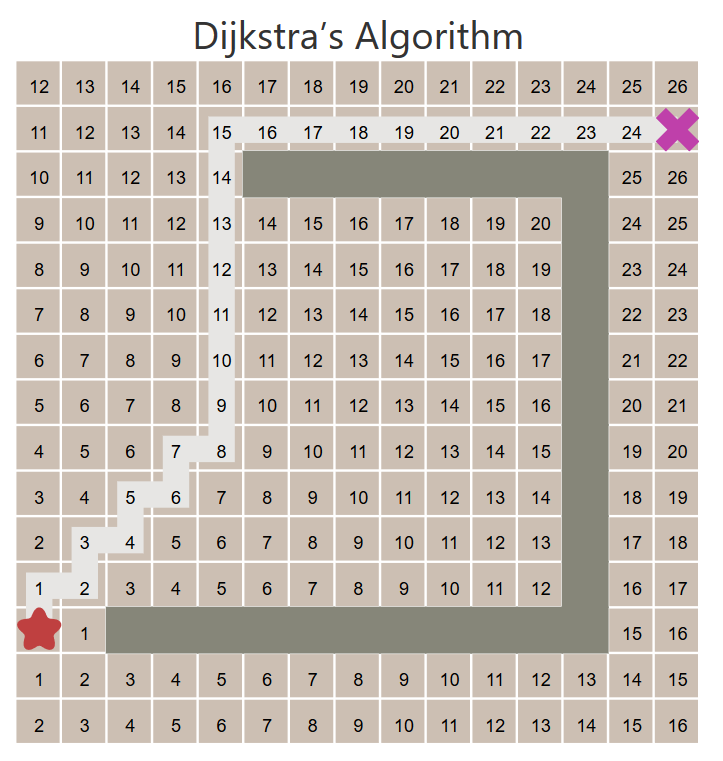
\includegraphics[width=1\textwidth]{djis3}
\end{minipage}
\begin{minipage}[c]{0.5\textwidth}
	\centering
    Después de la Búsqueda
	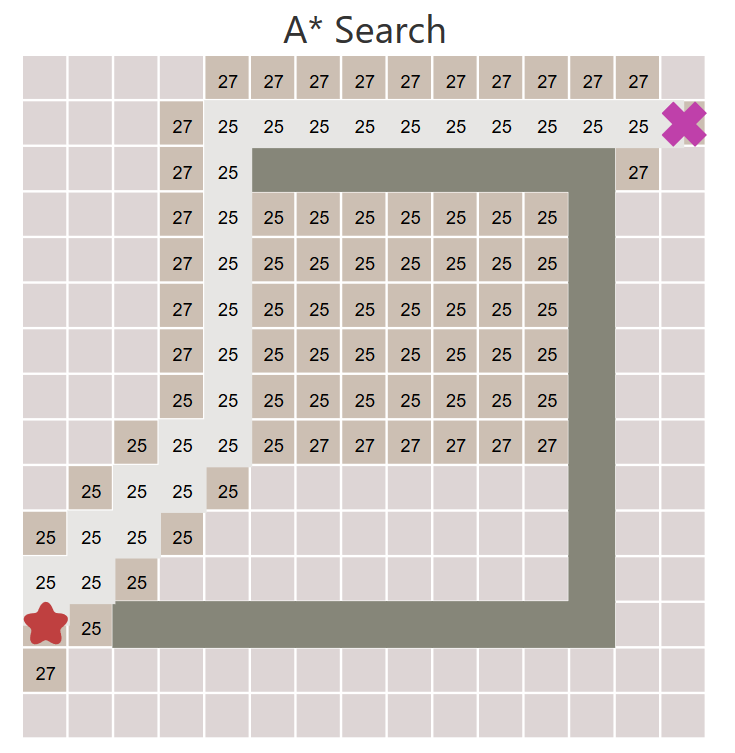
\includegraphics[width=1\textwidth]{A}
\end{minipage}
\begin{center}
\caption{\label{fig:A} Comparacion entre Dijkstra's y A*} 
Fuente: \textit{Introduction to A*}\cite{Red2016June}.
\end{center}
\end{figure}


\subsubsection{HEUTISTICAS}


Como vimos en A* usar heuristicas puede acelerar la búsqueda del camino, algunos ejemplos usados en la literatura son los siguientes.

\begin{enumerate}

\item \textit{Manhattan}: Explicada en la sección de A*. 

\item \textit{Octile}: Para los mapas que permiten movimiento diagonal, se usa con A* en estos mapas.

\begin{align*}
	Octile &= \sqrt{2}*m + (M-m) \\
	m &= min( \Delta x, \Delta y) \\
	M &= max( \Delta x, \Delta y)
\end{align*}

\item \textit{Differential}: \cite{goldberg2005computing}
 Se hace un paso de procesamiento previo calculando la distancia real desde todos los puntos a unas \textit{landmarks}\footnote{Puntos "importante" dentro del mapa, pueden ser cuellos de botella, posiciones predefinidas u otros}. Con esta información puedes calcular la heuristica para tener una estimación de la distancia entre el nodo $n_1$ y $n_2$ con todas las \textit{landmarks} L.

\begin{align*}
	Differential &= max(| d(n_1,l) - d(n_2,l) |),  \ l \in L \\
	d(n_x,l) &= distancia\ entre\ n_x\ y\ l
\end{align*}

Esto aproxima con la máxima distancia para evitar casos como que un \textit{landmark} este en medio de ambos nodos.

\item \textit{Dead-end}: \cite{bjornsson2006improved} Identifica areas que no tienen la solucion y les da un valor infinito. 
	
\item \textit{Gateway, canonical y portal}: \cite{bjornsson2006improved,sturtevant2009memory,goldenberg2010portal} Tres heuristicas que intentan separar el mapa en los cuellos de botella y precomputar movimientos entre los sectores creador

\end{enumerate}


\subsubsection{ABSTRACCIONES DE MAPA}







Como vimos, lo normal es representar el mapa en un tablero, existen algoritmos que toman este tablero y hacen abstracciones posteriores para encontrar soluciones de mayor nivel rápidamente, esto permite trabajar en grafos mas pequeños y después cortar el grafo original para buscar una solución. También permite tener una dirección aproximada mas rápidamente, lo cual puede permitir que el agente empiece su movimiento sin tener la solución completa.

Se tiene que tener claro que al encontrar una solución a un nivel mas alto tienes que tener seguridad que es una solución inferior, porque hacer \textit{backtracking} puede ser muy costoso.

\begin{enumerate}

\item \textit{HPA*}: \cite{botea2004near} Separa el mapa en sectores cuadrados, las conexiones entre sectores se identifican y son agregadas como nodos. Luego que se arman todas las capas que se decidieran, se puede buscar conectando el nodo origen y final a sus sectores y hacer el \textit{pathfinding} desde el nivel mas alto hacia abajo.

\item \textit{PRA*}: \cite{sturtevant2005partial} Recursivamente separa el mapa en bloques de $2x2$, hasta que el mapa esta representado por un solo nodo. Con el origen y el final conectados a una capa de abstracción se inicia el \textit{pathfinding} y se va bajando por la pirámide de abstracciones.

\item \textit{HAA*}: \cite{harabor2008hierarchical} Basado en HPA*, tiene dos cambios al anteriores, permite el uso de distintos tipos de terreno, como agua y bosque, que afectan a que unidades pueden atravesarlo. Ademas permite usar unidades de tamaño diferente, las unidades comunmente vistas son de una celda, en este caso se puede encontrar el camino para unidades que usan 4, 9 o mas, celdas.

\item \textit{Block A*}: \cite{yap2011block} Usando un tamaño predefinido de $m * n$, se precomputan todas las posibles combinaciones de terreno que pueden existir en ese tamaño de bloques, en ves de expandir por nodo, se expande cada bloque.


\end{enumerate}

%\subsubsection{OTROS}

%\begin{itemize}

%\item 

%\end{itemize}

%\subsubsection{PATHFINDING DE VARIOS AGENTES}



\newpage
\secnumbersection{PROPUESTA DE SOLUCIÓN}


\newpage
\secnumbersection{VALIDACIÓN DE LA SOLUCIÓN}


\newpage
\secnumbersection{CONCLUSIONES}



\newpage
\secnumberlesssection{ANEXOS}



\newpage
% Bibliografía estilo IEEE con las citas "especiales".
\bibliographystyle{IEEEtranSN}
\bibliography{bibliografia}{}

\end{document}
